\section{System Overview}
\label{sec:overview}

%An intuitive solution for the \emph{Text-to-Constraints} problem is to prompt an LLM with the entire document, schema, and sample records, asking it to extract constraints directly.
%\system\ also supports this mode, but in practice, it can be brittle when schemas are large or texts are long and loosely structured. Relevant text is usually scattered throughout the document, much of the content is unrelated to data or constraints, and so the prompt must simultaneously detect constraint-relevant text, align it with the schema, and generate constraints. Document-level processing also offers limited traceability, as identifying which part of the text justifies a given constraint is itself a separate task.

This section presents \system, our proposed framework for the Text-To-Constraints problem. 

Intuitively, one can address this problem by using an LLM with a general prompt that includes the entire document, the dataset schema, and instructions for extracting constraints. However, document-level prompting faces structural challenges on some inputs, as relevant statements may be scattered across the text, much of the content may be unrelated to data quality, and the model must jointly identify relevant parts of the text, align them with the schema, and construct valid constraints. 
\DIFdelbegin \DIFdel{The outputs of this }\DIFdelend \DIFaddbegin \DIFadd{Such }\DIFaddend document-level \DIFdelbegin \DIFdel{mode }\DIFdelend \DIFaddbegin \DIFadd{outputs }\DIFaddend also offer less direct traceability, since linking a generated constraint back to the supporting text is itself a separate step.
\altic{[R1-O4] Tornar o argumento de (falta de) rastreabilidade mais preciso e menos absoluto. O revisor não comprou ``LLM não é rastreável''. Reformular: não é que o LLM seja incapaz, e sim que o modo document-level NÃO produz por construção o vínculo sentença->constraint; ele exige um passo extra de atribuição. Citar/discutir a alternativa do revisor (pipeline iterativo de sumarização antes do mapeamento) e dizer por que o modo sentence-level já entrega essa rastreabilidade de graça.}

We therefore \DIFdelbegin \DIFdel{consider an alternative mode and }\DIFdelend decompose the problem into a pipeline that operates \DIFdelbegin \DIFdel{primarily }\DIFdelend at the sentence level, processing each sentence individually. This design provides fine-grained traceability, since it links each constraint to the specific sentence that justifies it, and allows each component of the pipeline to be tuned independently.

\DIFdelbegin \DIFdel{We design }%DIFDELCMD < \system%%%
\DIFdel{\ to support these two modes, and our experiments in Section~\ref{sec:experiments} show that sentence-level processing is the more robust choice overall, particularly when traceability is important. %DIF < although document-level extraction can still perform well on some datasets.
}\DIFdelend \system\ takes as input a document in natural language and a relational dataset and outputs sentence--constraint pairs\DIFdelbegin \DIFdel{in sentence-level mode, or a flat set of constraints in document-level mode}\DIFdelend . Figure~\ref{fig:pipeline} outlines the pipeline.

\begin{figure}[!ht]
\vspace{-10pt}
\centering
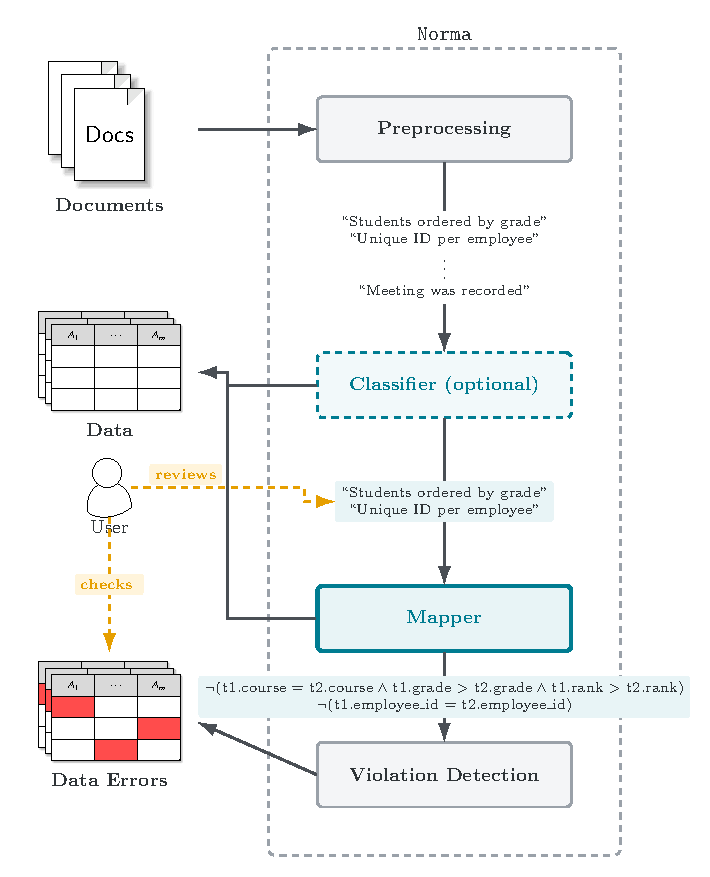
\includegraphics[width=\columnwidth]{diagramas/pipeline_norma.pdf}
%\caption{The \system\ pipeline.}
\vspace{-10pt}
\caption{Overview of the \system\ pipeline. \DIFdelbeginFL \DIFdelFL{Solid arrows show sentence-level mode. The dashed blue arrow shows document-level mode. }\DIFdelendFL Blue components represent the novel contributions presented in this paper.}
\label{fig:pipeline}
\vspace{-10pt}
\end{figure}

\smallskip\noindent\textbf{Preprocessing.}
We start from documents (e.g., PDF files) and produce a normalized text representation.
This step can be noisy, as headers and footers often leak into the body, line breaks split tokens, footnotes disrupt reading order, and lists get flattened into fragments that hinder sentence boundary detection. Since our goal is Text-to-Constraints 	rather than document conversion, we treat preprocessing as input preparation and do not focus on it in this work. We run an automated pipeline covering text extraction,	dehyphenation, whitespace normalization, and sentence segmentation, followed by minimal manual cleanup.


\smallskip\noindent\textbf{Constraint classifier.}
Given the sentences from preprocessing, a lightweight classifier can optionally identify those that likely express checkable constraints, filtering out content that surely has nothing to do with data quality constraints.  Since constraints missed at this stage cannot be recovered downstream, we prioritize recall at this stage. False positives can still be ruled out by the mapper, which applies a more expressive classification strategy internally.\altic{[R3-O5] Referência adiantada confusa: o ``mapper'' ainda não foi definido aqui. Aplicar a correção sugerida pelo próprio revisor: trocar ``...ruled out by the mapper, which applies a more expressive classification strategy internally'' por ``...ruled out by the mapper (which we define next)'', evitando descrever a ``estratégia mais expressiva'' antes de o leitor saber o que é o mapper.} When no classifier is used, all sentences are passed directly to the mapper. A user can optionally be involved at this stage, reviewing and correcting the set of classified sentences before proceeding to mapping. We describe the classifier details in Section~\ref{sec:classifier}.


\smallskip\noindent\textbf{Constraint mapper.}
The mapper is the central and most complex component of \system. It takes each sentence, optionally pre-filtered by the classifier, and produces a denial constraint grounded in the dataset schema. Some mapper implementations have an internal classification step that uses schema-based information to decide whether a sentence yields a valid constraint before attempting to construct one.
The mapper must interpret natural language, align it with schema elements, and synthesize a constraint with correct violation semantics. Outputs that fail syntactic validation are rejected, and sentences that yield no valid constraint are excluded from the final output. \DIFdelbegin \DIFdel{In document-level mode, the mapper receives the entire document in a single call and
extracts all constraints at once, using similar prompting strategies and schema-grounded instructions as in sentence-level mode. }\DIFdelend We describe the different mapper implementations in detail in Section~\ref{sec:mapper}.


\smallskip\noindent\textbf{Violation detection.}
Each constraint is validated by compiling it into a SQL violation query and executing it on the target relation \DIFdelbegin \DIFdel{. In sentence-level mode, each constraint is also }\DIFdelend \DIFaddbegin \DIFadd{(Section~\ref{sec:mapper:sql}), and it is }\DIFaddend linked back to the sentence that produced it. \system\ returns the violating tuples to the user for further inspection. DC violation detection is a well-studied problem, with specialized systems available for large-scale consistency checks~\cite{facet2021,liu2024rapidash,youri2024}.
\altic{[R1-O6] Justificar a escolha de compilar para query SQL de violação em vez de usar engines especializadas de validação de DC. O parágrafo já cita facet/rapidash/youri; explicitar que SQL/DuckDB é só a implementação do protótipo e que as engines de DC são uma alternativa drop-in para escala, respondendo diretamente à pergunta do revisor.}

